\chapter{EXPERIMENTOS E RESULTADOS[EXPLICAR FIGURAS]}
\label{experimentos}
\begin{comment}
    

\emph{Questão a ser respondida pelos Experimentos e Resultados: O que foi encontrado?}
A seção de experimentos e resultados organiza e simplifica as descobertas da pesquisa para os leitores.

Concentre-se nos detalhes que são mais relevantes para avaliar o que foi estudado.
Faça comparações e descreva tendências quando apropriado (por exemplo, esse método teve acurácia melhor que aquele outro).
Utilize gráficos, tabelas, figuras para ajudar na apresentação dos resultados.
Evite qualquer interpretação ou explicação para os resultados.

Nesse capítulo é interessante ter uma seção falando sobre limitações que foram encontradas durante o projeto. Entretanto, a ideia não é justificar o que não deu tempo de fazer, mas sim elencar possíveis trabalhos futuros que essas limitações derivam.

É muito relevante colocar artigos e ou congressos que o projeto foi publicado e apresentado.
\end{comment}
Foram feitos testes para implementar a parte simulada proposta, sendo utilizado o manual \cite{turtlebot3_manual} e pacotes \cite{turtlebot3_github} disponíveis pelo grupo ROBOTIS, tornando o desenvolvimento desta parte rápido. A utilização e desenvolvimento dos projetos ROS2 dentro do Docker foi facilitada pela utilização de workflows no GitHub, onde as imagens de teste foram automaticamente construídas e publicadas como pacotes no repositório, o que reduziu o tempo do processo de construir as imagens localmente, que demorava de 20+ minutos para no máximo 5 minutos, além de também as disponibilizar para outros usarem.

%O erro é o \cite do github
%Foram feitos testes \cite{github_tcc_docker} para implementar a parte simulada proposta, sendo utilizado o manual \cite{turtlebot3_manual} e pacotes \cite{turtlebot3_github} disponíveis pelo grupo ROBOTIS, tornando o desenvolvimento desta parte rápido. A utilização e desenvolvimento dos projetos ROS2 dentro do Docker foi facilitada pela utilização de workflows no GitHub, onde as imagens de teste foram automaticamente construídas e publicadas como pacotes no repositório, o que reduziu o tempo do processo de construir as imagens localmente, que demorava de 20+ minutos para no máximo 5 minutos, além de também as disponibilizar para outros usarem.

Houve certas dificuldades para integrar o ROS2 dentro do contêiner Docker com o ROS2 nativo, que lidaria com a simulação Gazebo. Foi descoberto que o middleware utilizado por padrão pelo ROS2 Humble, FastDDS, não interage de forma consistente com Docker. Ele era capaz de compartilhar os tópicos entre os ambientes, mas causava falha na publicação e recebimento de mensagens, não mostrando nenhuma.

Para solucionar isso, o FastDDS foi substituído por outro middleware disponível para ROS2 Humble, CycloneDDS, o qual foi utilizado especificamente no contêiner Docker.

\begin{figure}[htb]
    \centering
    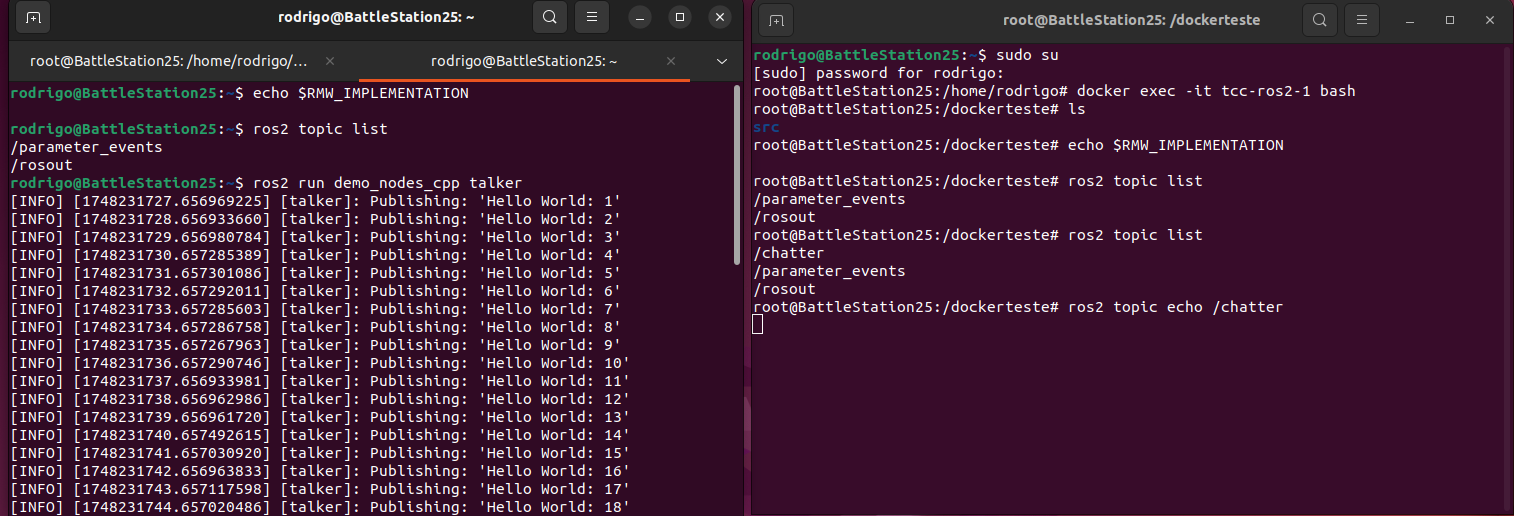
\includegraphics[width=1\linewidth]{Figures/TestePadraoFalha.png}
    \caption{Falha utilizando RMW padrão (FastDDS)}
    \label{fig:enter-label}
\end{figure}
\begin{figure}[htb]
    \centering
    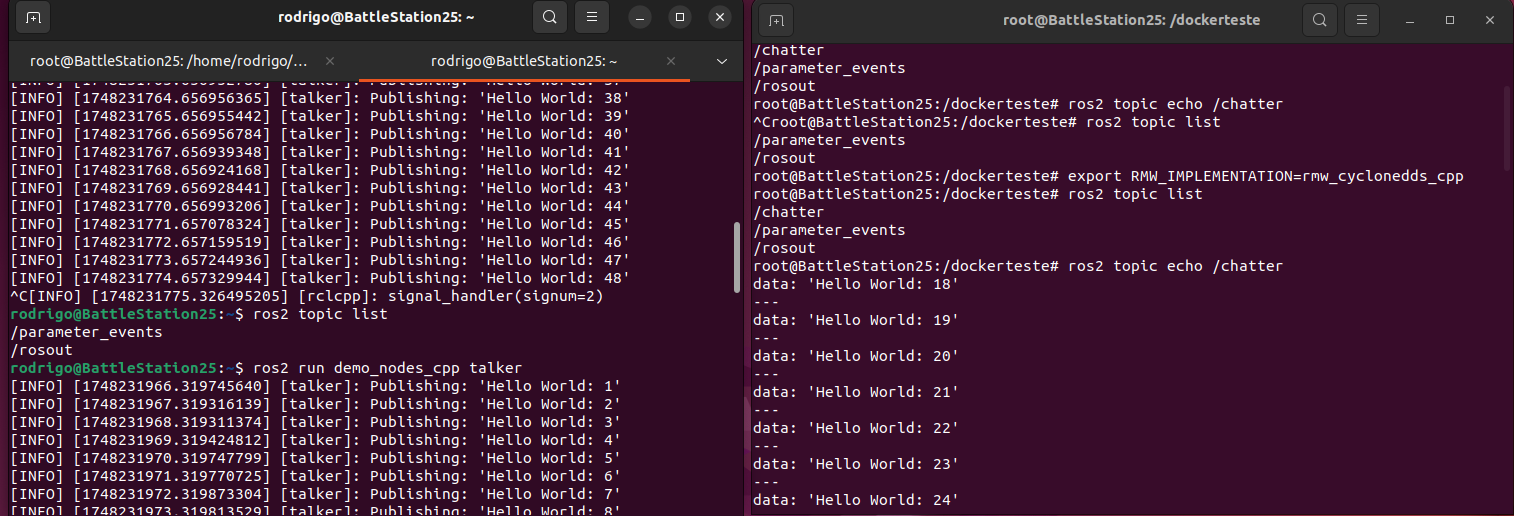
\includegraphics[width=1\linewidth]{Figures/TesteCycloneSucesso.png}
    \caption{Sucesso utilizando RMW CycloneDDS }
    \label{fig:enter-label}
\end{figure}
\begin{figure}[htb]
    \centering
    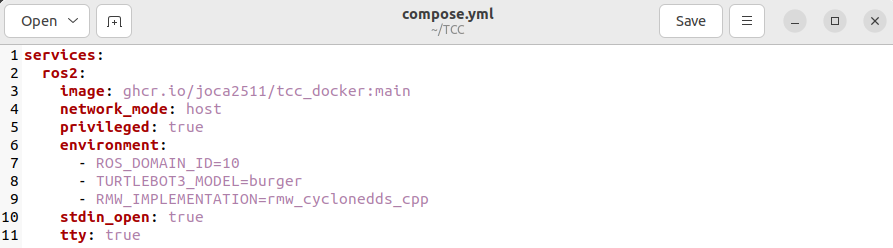
\includegraphics[width=1\linewidth]{Figures/ComposeFinal.png}
    \caption{Compose proposto para testes}
    \label{fig:enter-label}
\end{figure}
\begin{figure}[htb]
    \centering
    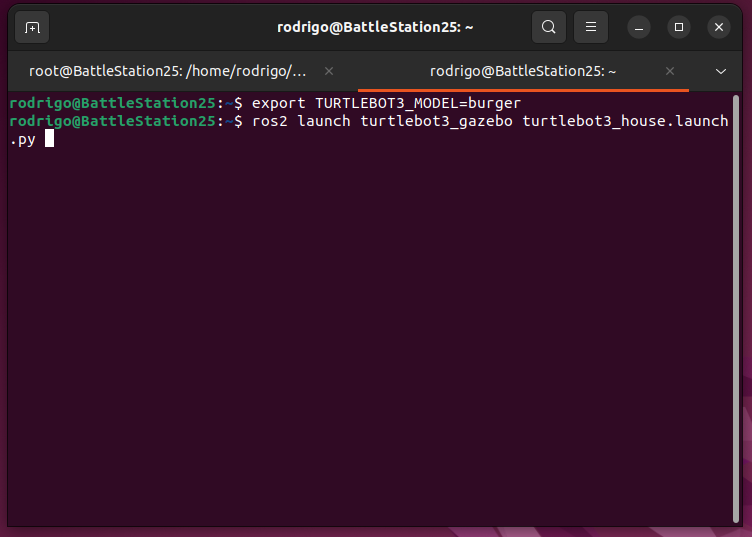
\includegraphics[width=1\linewidth]{Figures/SimulacaoGazeboLancada.png}
    \caption{Simulação Gazebo é lançada pelo host}
    \label{fig:enter-label}
\end{figure}
\begin{figure}[htb]
    \centering
    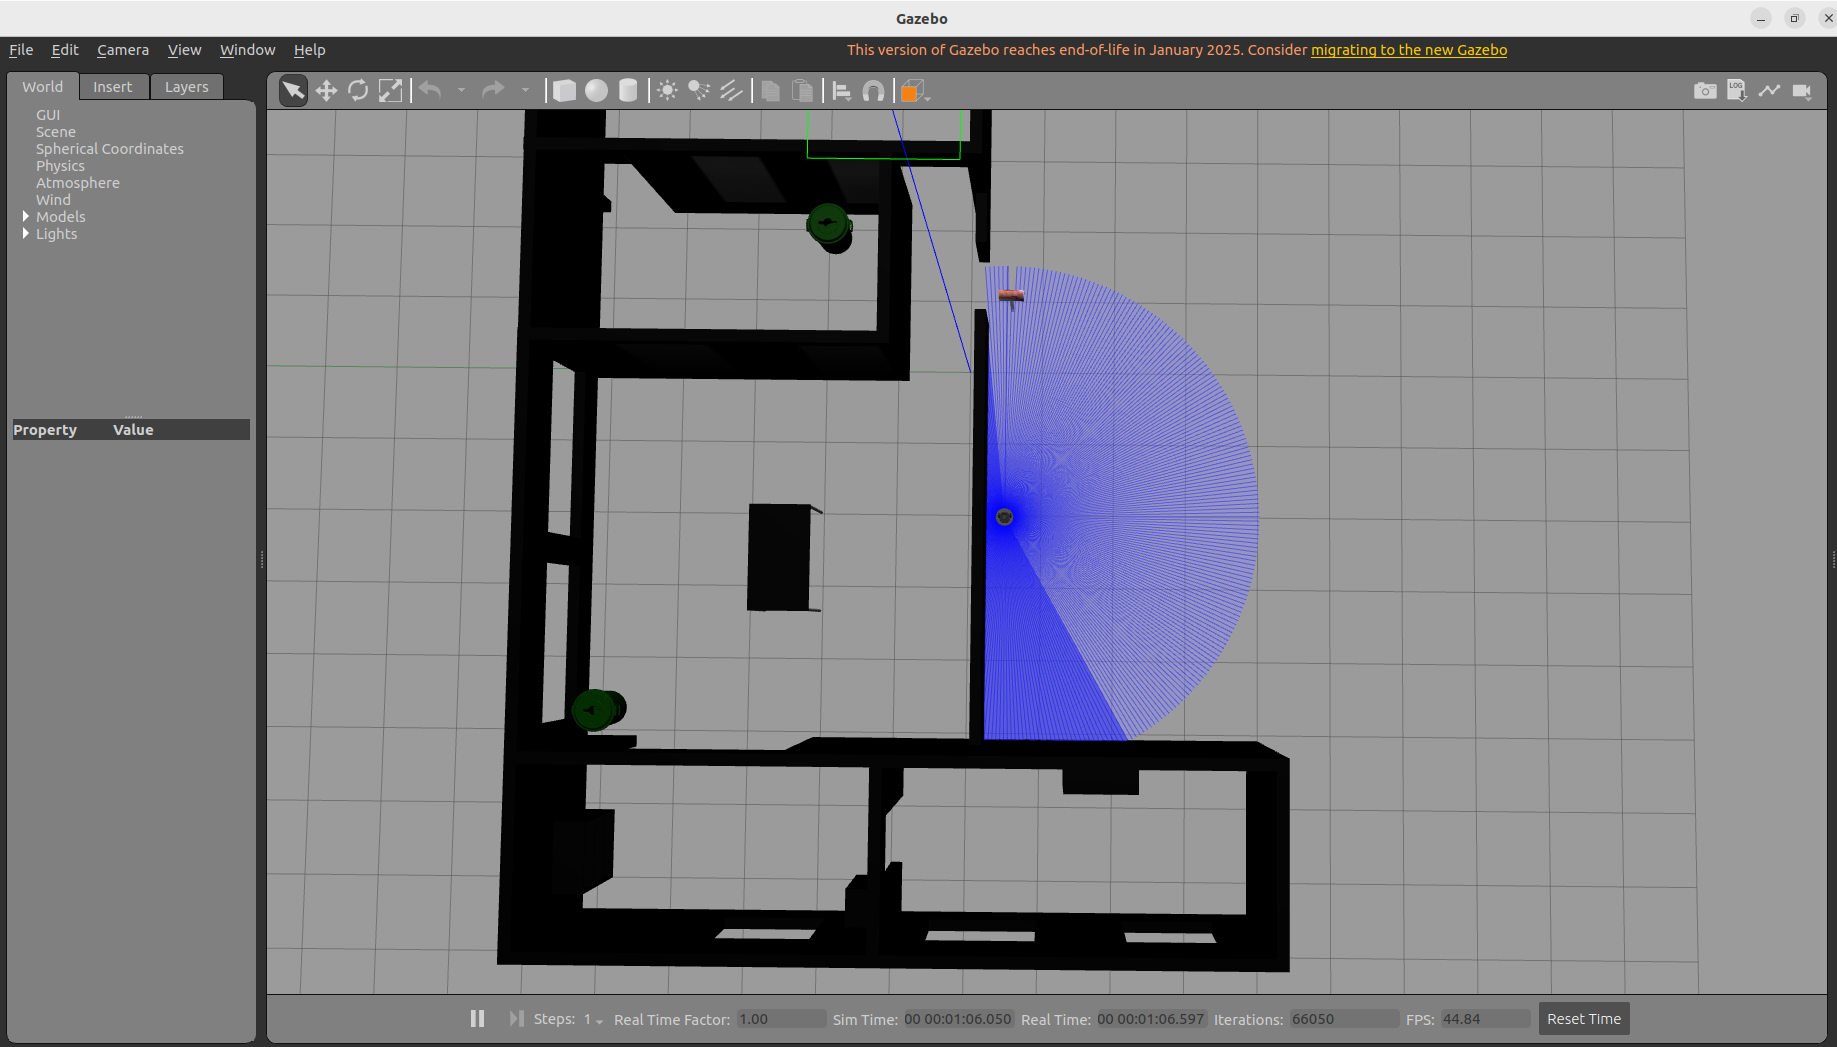
\includegraphics[width=1\linewidth]{Figures/GazeboLancado.png}
    \caption{Aparência inicial da simulação Gazebo}
    \label{fig:enter-label}
\end{figure}
\begin{figure}[htb]
    \centering
    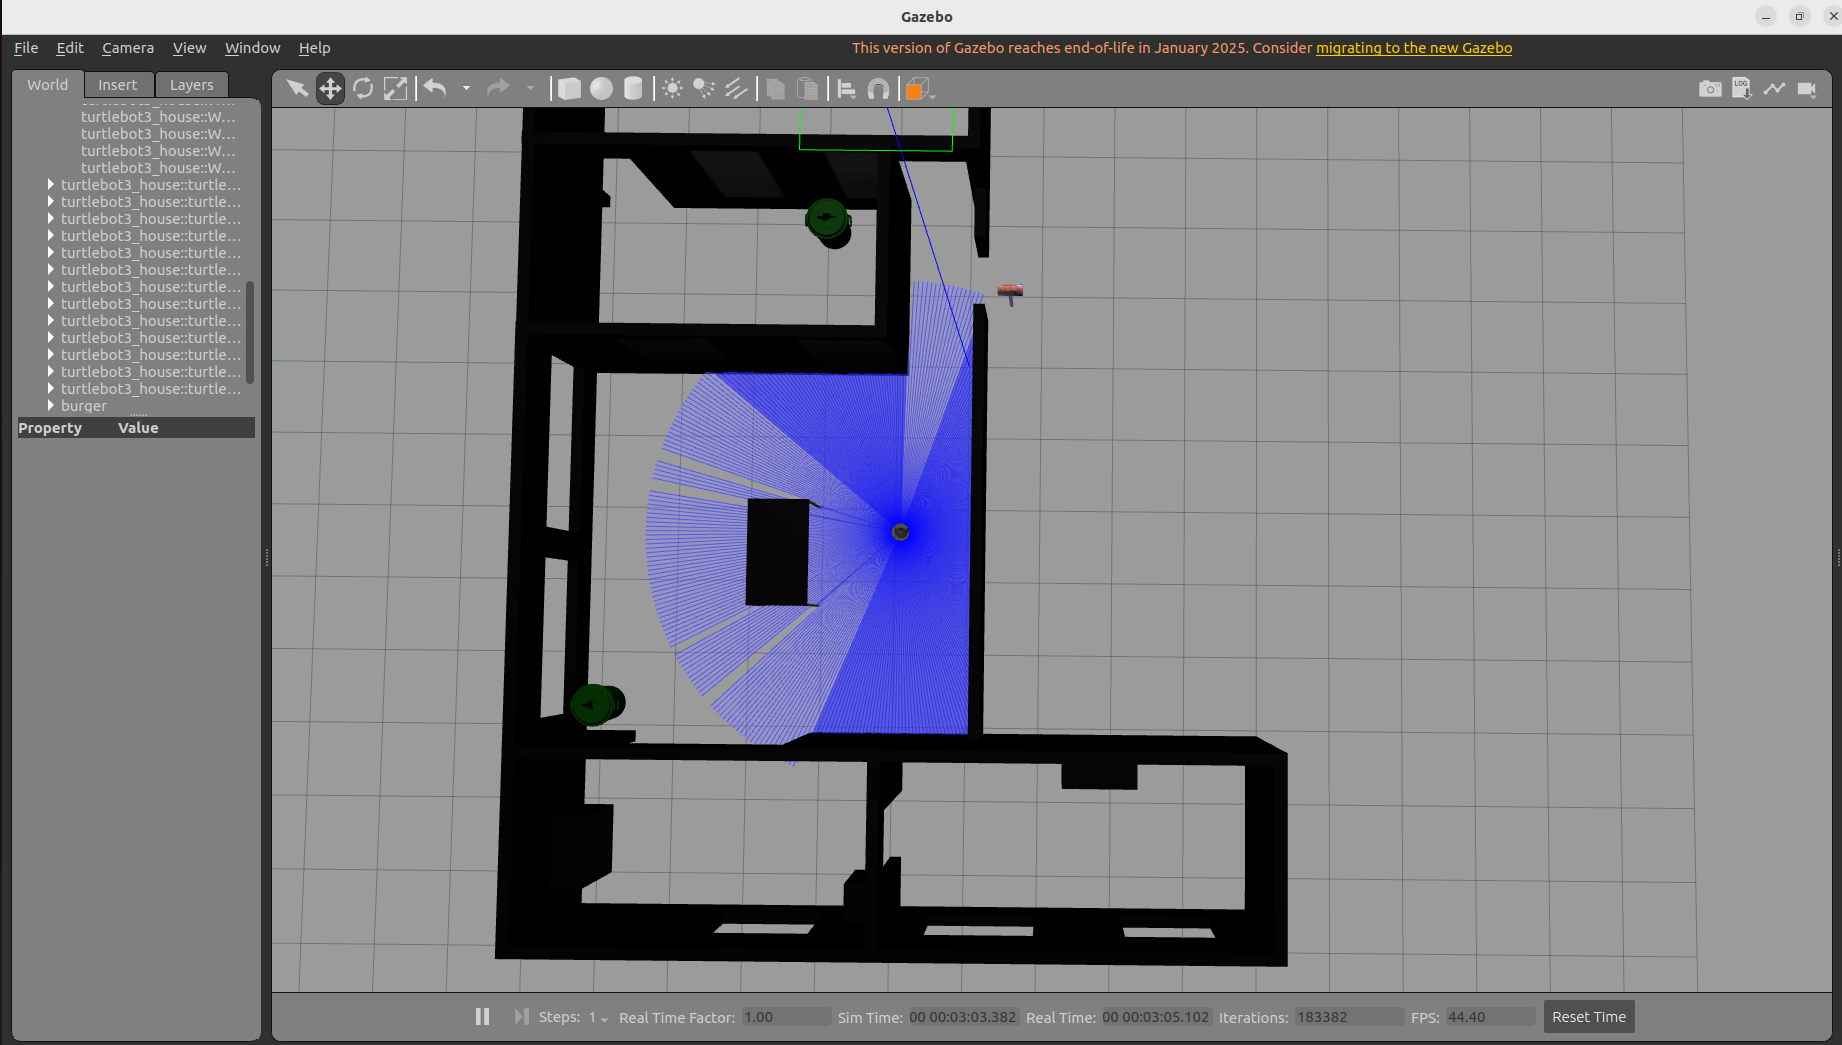
\includegraphics[width=1\linewidth]{Figures/BurgerMovido.png}
    \caption{Turtlebot3 Burger é movido para dentro da casa}
    \label{fig:enter-label}
\end{figure}
\begin{figure}[htb]
    \centering
    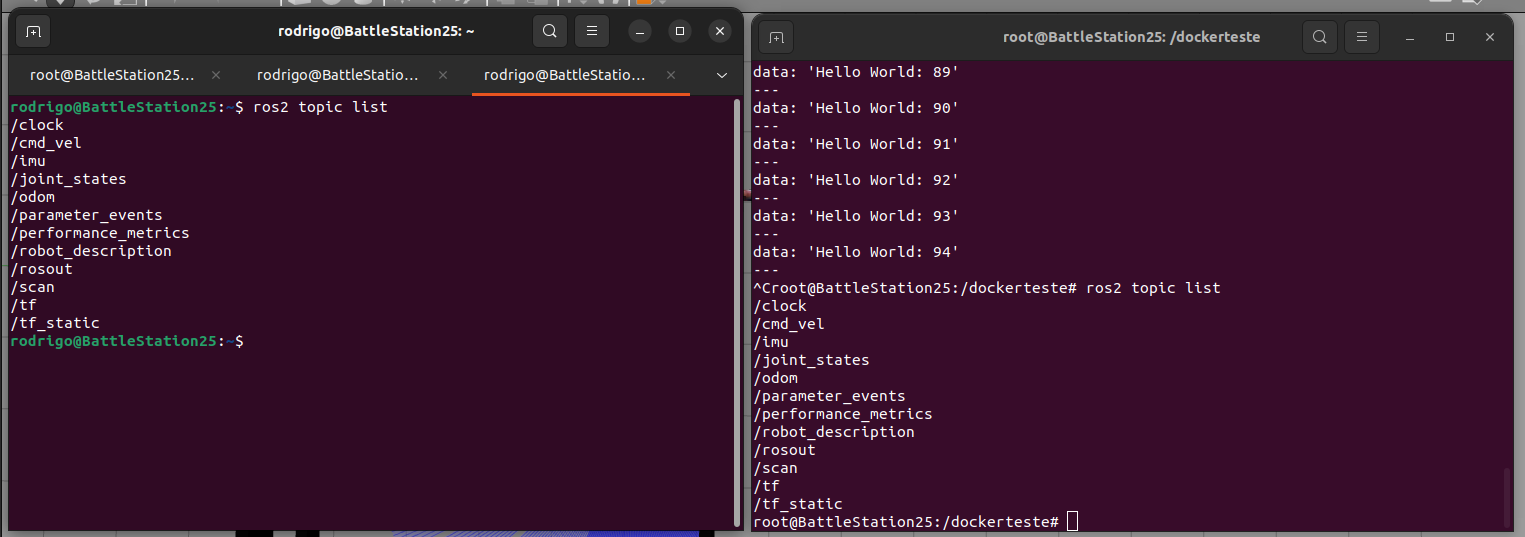
\includegraphics[width=1\linewidth]{Figures/DockerAdquireTopicos.png}
    \caption{ROS2 Humble dentro do Docker adquire os novos tópicos}
    \label{fig:enter-label}
\end{figure}
\begin{figure}[htb]
    \centering
    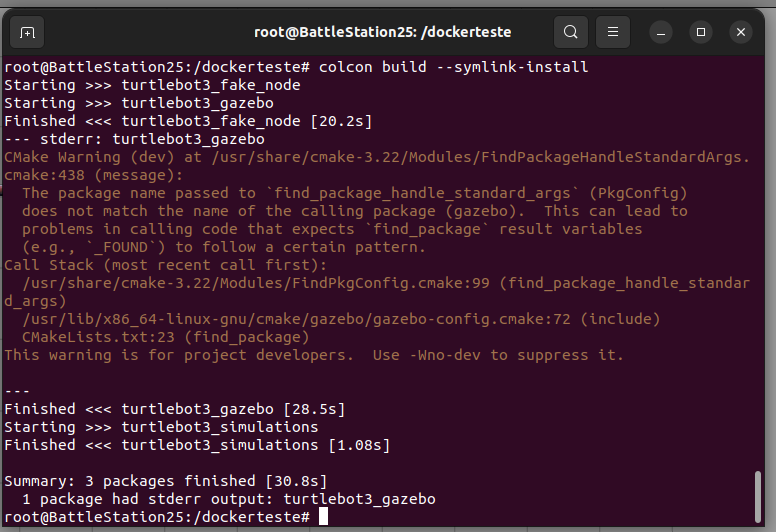
\includegraphics[width=1\linewidth]{Figures/DockerBuildaProjetos.png}
    \caption{ROS2 Humble dentro do Docker builda projetos}
    \label{fig:enter-label}
\end{figure}
\begin{figure}[htb]
    \centering
    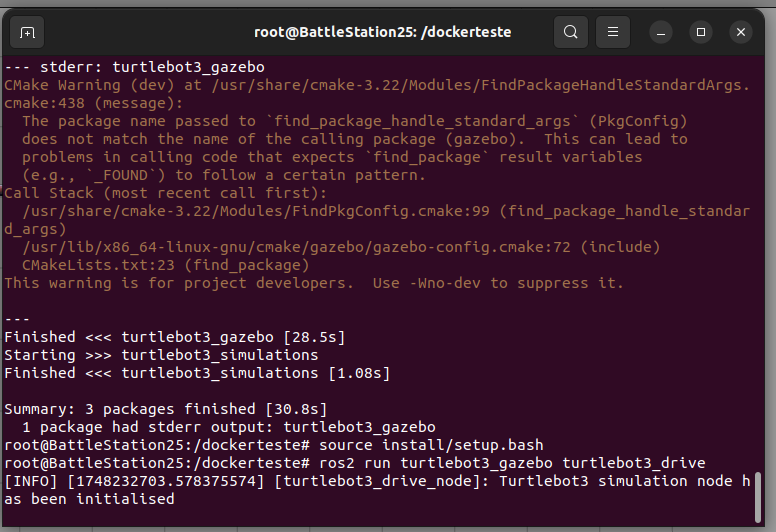
\includegraphics[width=1\linewidth]{Figures/DockerRodaProjetoDrive.png}
    \caption{ROS2 Humble dentro do Docker roda projetos para movimentação do robô dentro da simulação Gazebo presente no host}
    \label{fig:enter-label}
\end{figure}
\begin{figure}[htb]
    \centering
    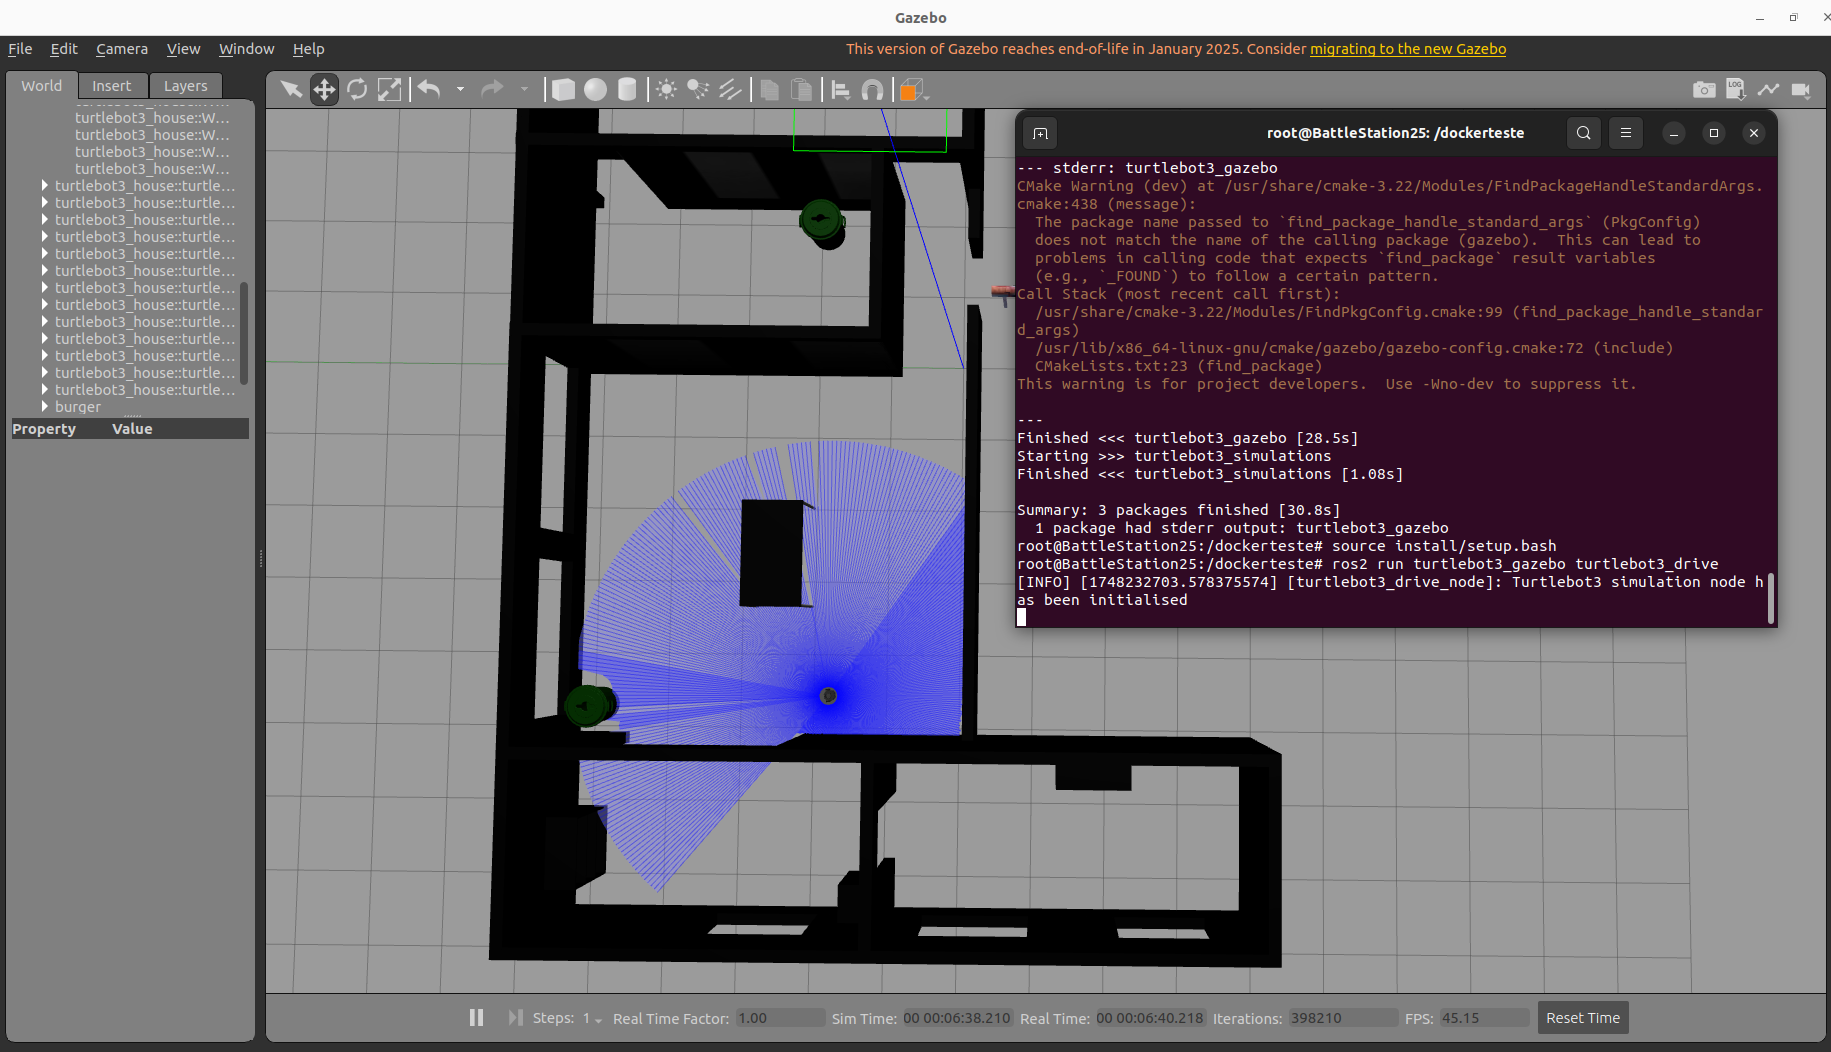
\includegraphics[width=1\linewidth]{Figures/DockerMovimentaRobo1.png}
    \caption{Turtlebot3 Burger é movimentado pelo ROS2 Humble presente dentro do conteiner Docker}
    \label{fig:enter-label}
\end{figure}
\begin{figure}[htb]
    \centering
    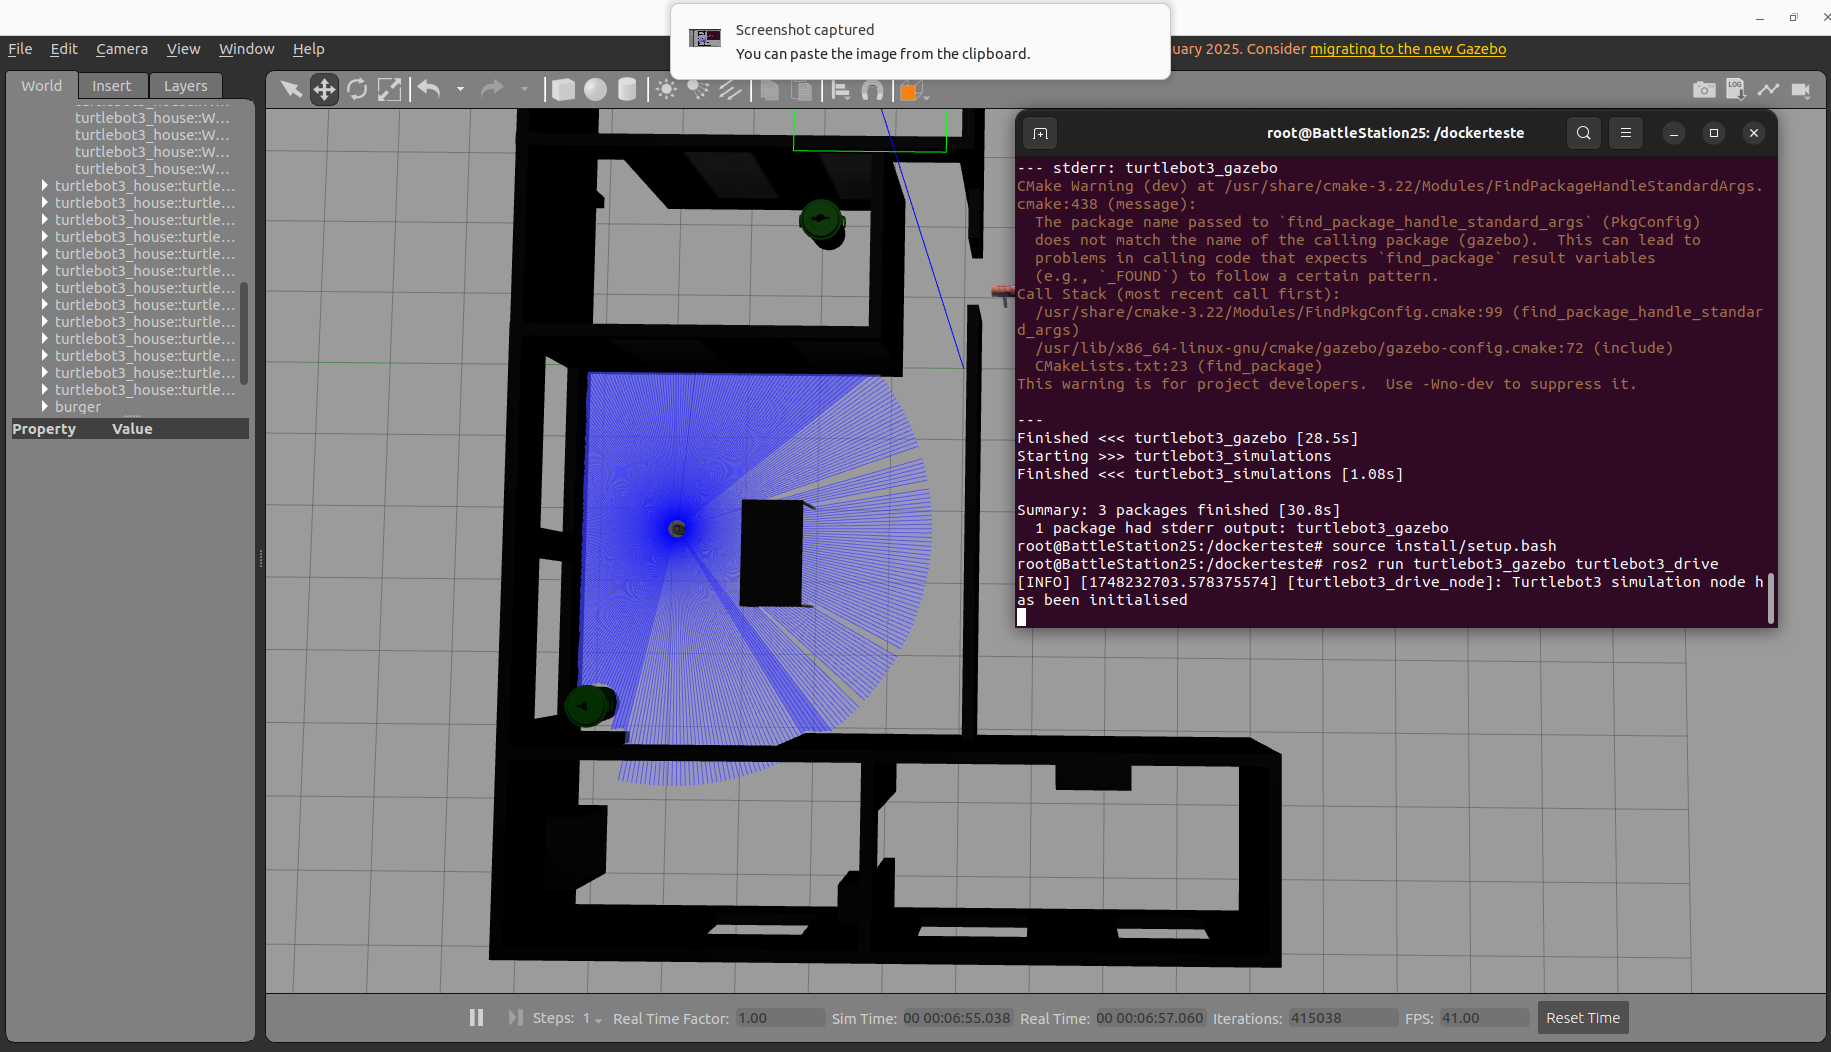
\includegraphics[width=1\linewidth]{Figures/DockerMovimentaRobo2.png}
    \caption{Turtlebot3 Burger é movimentado pelo ROS2 Humble presente dentro do conteiner Docker}
    \label{fig:enter-label}
\end{figure}

